\begin{center}
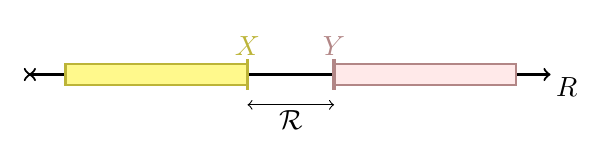
\begin{tikzpicture}[scale=.55]

    % Number line
    \draw[thick,->] (-6,0) -- (6,0);
    \draw[thick,<->] (-6,0) -- (-6.05,0); % left arrow tip

    % X region (yellow)
    \filldraw[
        fill=yellow!45,
        draw=yellow!70!black,
        thick
    ] (-5.2,-0.25) rectangle (-1,0.25);

    % Y region (pink)
    \filldraw[
        fill=pink!35,
        draw=pink!70!black,
        thick
    ] (1,-0.25) rectangle (5.2,0.25);

    % Boundary markers
    \draw[very thick,yellow!70!black] (-1,-0.35) -- (-1,0.35);
    \draw[very thick,pink!70!black] (1,-0.35) -- (1,0.35);

    % Labels
    \node[yellow!70!black] at (-1,0.65) {$X$};
    \node[pink!70!black] at (1,0.65) {$Y$};

    % Gap label
    \draw[<->] (-1,-0.7) -- (1,-0.7);
    \node at (0,-1.05) {$\mathcal{R}$};

    % Real numbers label
    \node[right] at (5.9,-0.3) {$\mathbb{R}$};

\end{tikzpicture}
\end{center}
